\documentclass[12pt,letterpaper]{article}

\usepackage[utf8]{inputenc}
\usepackage{amsmath}
\usepackage{amsfonts}
\usepackage{amssymb}
\usepackage{graphicx}
\usepackage{algorithm2e}

\author{Andrew Matteson}
\title{CSCD 320 Algorithms Report}
\date{\today}

\pagestyle{myheadings}
\markright{Andrew Matteson  00495489 \hfill}

\begin{document}

\maketitle

\section{Abstract}


With tax season just around the corner, our president has asked that the top 10,000 richest people have their taxes doubled checked. There is one issue though, the government was stingy during its last budget meeting and has only been given a computer with enough room to load 10,000 people onto its main memory. To achieve this goal,  this paper will discuss how this is done using a min heap.

\section{Introduction}

Even with the increasing amount of affordable RAM, data sets can sometimes be so large that there is no feasible way to load it all on main memory. By coming up with effective ways to get around this issue and still maintain speed and effectiveness, we can analyze enormous files without too much of this concern.

Our particular problem consists of simulating a limited main memory to 10,000 items. Then as we read in each additional number we have to decide if it should replace something already in our main memory, or discard it.  Our next section will look at the algorithm used to solve this problem. Then we will compare results using various file sizes. Lastly, the paper will conclude with other possible experiments to run.


\section{Algorithm}
This is broken up into quick summary of the algorithm and then it delves into the particular algorithms used to solve the problem.

\subsection{Quick summary}
The following set of directions represents the core idea of how our problem was solved.
\begin{enumerate}
\item Fill up the memory with the first 10,000 numbers and then min heapify the list.
\item Read in another number and compare it with the root, if it is larger, replace the root with this number then heapify this list.
\item repeat the previous step until every number has been read in.
\end{enumerate}



\subsection{ Detailed algorithm}
Now that we have the general approach, lets delve deeper and analyze precisely how each step was achieved.
\begin{enumerate}
\item I made a global counter variable to keep track of the index of each read in value. 
\item Read in the first 10,000 numbers into the array, then run array through the Build\_Min\_Heap function. This method works from the leafs nodes up constructs the array into a min heap.


\begin{algorithm}[H]
	\NoCaptionOfAlgo
	{\bf Build\_Min\_Heap( heapArray)} \\
	\For{$i = MinHeapSize \to 0$}
	{
		Min\_Heapify( heapArray, i) \;
	}
\end{algorithm}

where the Min\_Heapify algorithm is the following:

\begin{algorithm}[H]
	\NoCaptionOfAlgo
	{\bf Min\_Heapify( heapArray, i) }\\
	smallest = 0 \;
	left = 2 * i \;
	right = 2 * i + 1 \;
	\eIf{ left $<=$ MinHeapSize and \\ heapArray$[$left$]$.value $<$ heapArray$[i]$.value}
	{
		smallest = left\;
	}{
		smallest = i \;
	}
	
	\If{$right <= MinHeapSize$ and \\ heapArray$[$right$]$.value $<$ heapArray$[$smallest$]$ }
	{
		smallest = right\;
	}
	
	\If{smallest $!=$ i}
	{
		tempVal = heapArray[i].value \;
		tempIndex = heapArray[i].index \;
		
		heapArray[i].value = heapArray[smallest].value \;
		heapArray[i].index = heapArray[smallest].index \;
		
		heapArray[smallest].value = tempVal \;
		heapArray[smallest].index = tempIndex \;
		Min\_Heapify(heapArray, smallest)\;
	}
\end{algorithm}

	\item Now that we have built our min heap array, for every next value in the text file, compare its value with the root node of our Min Heap array. If it is larger than it, replace the root with this larger value. Then run Min\_Heapify( heapArray, 1). This will fix our heap to guarantee it is still a min heap.
	\item Continue the last step until every number is read in. Then the numbers in the min heap will be the top 10,000 numbers in the file.


\end{enumerate}



\section{Implementation}
It was pretty clear from the start that we wanted to use the idea of a heap for this project. The difficulty lay in deciding whether to use a min heap or a max heap. The major issue with using a max heap is we don't have the easy comparison with the root when we start reading in values one at a time. This flaw made min heap the clear winner.

Since the goal of this paper was to optimally use limited main memory, I chose C as my language of choice due to its speed and ease.  I first made multiple text files to simulate various list sizes and orders.  I created a 100 million, 10 million and 1 million number files where one set was created using the random library and another file was created sequentially starting at 1 and ascending. The reason for creating this sequential file was to create an upper bound for time since it has to go through most steps within the code. This is due to every new number being read in as larger than all the previous numbers, thus making us have to replace the root of the list and heapify it all the way down to a leaf node.

I used an array of structs of size 10,000 to simulate our limited main memory constraint. Inside each struct was two integer values, one for the actual value and another to keep track of the index which that value occurs.






\section{Performance}
This simulation was run  Ubuntu 12.04.2 on a virtual machine given 2 cores of 3.2 GHz Intel Core i3, and 2800 MB of 1333MHz DDR3 RAM. I ran each text file 5 times and averaged the runs to try and reduce the scheduler spoiling a particular run.

As we can see from the table, the time it took for the algorithm to go through the sorted number list was nearly double that of the random number list. This isn't too surprising as we expected the sorted list to take significantly longer due to the fact it has to take each number and bring it all the way from the root node to a leaf node.


\begin{figure}
\begin{center}
\begin{tabular}{|r | c | c | c | c | c| c|}
\hline
							& \textbf{Run 1}		&\textbf{Run 2}   	&\textbf{Run 3}		&\textbf{Run 4}	&\textbf{Run 5}	&\textbf{Avg} \\
						\hline 
100 million (random)	&26.46		&26.12		&26.02		&28.22	&27.93	&26.95 \\
100 million (ordered)	&52.35		&51.32		&50.92		&50.98	&51.27	&51.368\\
10 million (random)	&2.28	  		&2.04			&1.99			&1.94		&2.04		&2.058\\
10 million (ordered)	&4.89			&4.58			&4.55			&4.5		&4.83		&4.67\\
1 million (random)	     &0.23			&0.2			&0.2			&0.2		&0.2	     &0.206\\
1 million (ordered) 	&0.47			&0.47			&0.5			&0.43		&0.42		&0.458 \\
\hline
\end{tabular}
\caption{Time sheet of each run.}
\end{center}
\end{figure}

The graphs show  a side by side comparison with each sized input text file.


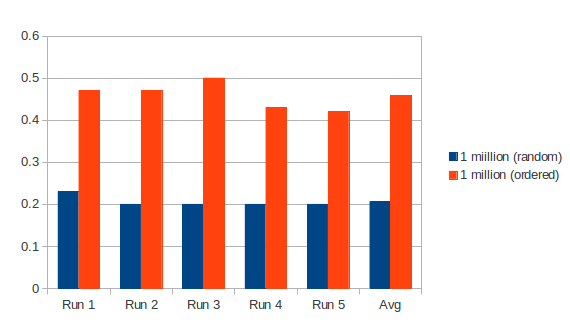
\includegraphics[scale=.5]{1mill.png}

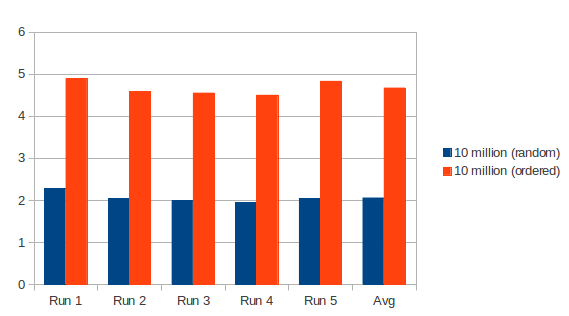
\includegraphics[scale=.5]{10million.png}

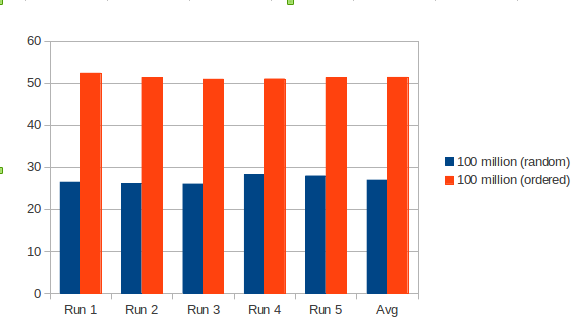
\includegraphics[scale=.5]{100million.png}






\section{Conclusion}

Not only were we able to achieve our goal of finding the top 10,000 items in the list with only enough room to hold 10,000 people in main memory, we did it in blazing speed. It would have been interesting to run this algorithm in other programming languages to see which one produced the fastest result. I have a feeling that it will be hard to find a language that will do it faster than C though. 

Another addition that could have been done was to make another input text file, but instead made it in descending order which would have given me a lower bound in terms of time. Thus we could have ended with a lower bound with descending ordered file, average time with random file and upper bound with ascending file.






\end{document}